% Chapter 1: 绪论 (Introduction)
\chapter{绪论}

\section{研究背景和意义}

现实环境中的优化任务正面临高维、非线性及多模态等复杂挑战，这类NP-hard问题广泛存在于工程设计\cite{ibsa_ref1}、机器学习超参调优\cite{ibsa_ref3}以及生物信息学\cite{ibsa_ref15}等领域。面对庞杂的搜索空间，传统确定性算法过度依赖梯度信息，往往难以稳定地捕获全局最优解\cite{ibsa_ref4}。与此同时，互联网技术的普及引发了数据规模的爆发式增长，高维复杂数据渗透进医疗诊断\cite{ibsa_ref11}、路径规划\cite{ibsa_ref9}和金融服务\cite{ibsa_ref8}等各行各业。这类数据通常夹杂着大量冗余或无效信息，不仅加剧了存储与计算负担，还会干扰学习模型的表征能力，削弱预测精度\cite{ibsa_ref17}。

元启发式算法通过模拟自然界的生物演化、群体协同或物理规律进行随机寻优，凭借其无梯度依赖、部署灵活及全局搜索能力较强等优势，已成为求解复杂优化问题的有效方法\cite{ibsa_ref16}，在特征选择\cite{ibsa_ref50}、图像多阈值分割\cite{ibsa_ref45}及调度优化\cite{ibsa_ref48}等任务中均有广泛应用。例如，Harris Hawks算法在处理工程约束问题时表现出优异的收敛性\cite{ibsa_ref83}；黏菌算法则在多模态景观搜索中具备良好的鲁棒性\cite{ibsa_ref28}。这些工作不仅丰富了计算智能理论，也为解决实际工程痛点提供了可行路径。

尽管元启发式算法展现出巨大潜力，但现有研究仍面临若干瓶颈。首要挑战在于探索与开发行为的失衡\cite{ibsa_ref75}，这常导致搜索前期覆盖不足或后期陷入局部极值。以高维医学数据特征选择为例，指数级增长的搜索空间要求算法在维持诊断性能的同时，必须精准剔除冗余特征，否则会显著加重分类器的计算负担。其次，搜索策略的选择及参数设置往往过度依赖人工先验经验\cite{ibsa_ref65}，削弱了算法应对多变问题的适应力。例如在多阈值图像分割任务中，噪声干扰、灰度不均等因素使得搜索景观差异巨大，静态机制难以维持性能的一致性。此外，在计算昂贵优化场景下，真实评估成本极高，样本利用效率直接制约了优化成效\cite{he2023review}。如油藏产量优化、翼型设计等工程问题，单次评估往往涉及复杂的数值模拟，如果采样缺乏导向性，有限的计算资源将迅速枯竭。针对上述难题，本研究从精英信息挖掘、自适应策略调控及代理模型辅助等方面切入，探索元启发式算法的演化机理与应用路径。

从应用维度审视，高维特征选择、医学影像分割与昂贵工程优化虽形式各异，其核心诉求均指向了有限计算资源下的高效寻优。特征选择侧重于在离散空间压缩维度，力求提升模型的可解释性与诊断精度\cite{ibsa_ref50}；多阈值分割则需在连续灰度域内精准定位，直接关系到病灶提取的可靠性\cite{sbo_ref82,sbo_ref83}；而昂贵优化更强调每一次评估的实际价值，力求以最小的计算成本换取最优的决策方案\cite{liu2023airfoils,kumar2024optimization}。这三类场景精准对接了探索与开发平衡、策略自适应与样本效率提升这三大核心瓶颈，为本研究提供了典型应用场景。

研究复杂优化环境下的元启发式改进策略，兼具理论深度与工程价值。在理论层面，这有助于解析搜索行为的演化规律，完善多样性维持与自适应决策机制\cite{ibsa_ref75}。在应用层面，高效的寻优算法能显著降低实际生产中的计算开销。通过在医学特征选择中降低特征冗余度，可以增强辅助诊断的稳健性；在图像分割任务中，能够提升病灶边缘识别的精细度；而在昂贵工程设计中，则能大幅缩短设计周期，确保参数决策的科学性\cite{ibsa_ref49,sbo_ref79,kudela2022recent}。

\section{国内外研究现状}

\subsection{元启发式优化算法研究现状}

元启发式算法在求解复杂优化问题中表现出独特优势，其灵感源于对自然界生物行为或物理规律的工程模拟。按机制差异可将其划分为生物启发（如PSO\cite{ibsa_ref26}、GWO\cite{ibsa_ref81}）、进化计算（如GA\cite{ibsa_ref33}、DE\cite{ibsa_ref34}）、物理化学过程模拟（如SA\cite{ibsa_ref29}、EO\cite{ibsa_ref32}）以及人类行为模仿（如TLBO\cite{ibsa_ref37}、BSO\cite{ibsa_ref40}）等体系。近年来，HHO\cite{ibsa_ref83}、SCA\cite{ibsa_ref31}及RIME\cite{sbo_ref49}等新型算法相继问世，进一步拓宽了该领域的研究范畴。

目前的改进研究主要聚焦于自适应参数控制、异构策略融合及种群多样性维系，旨在提升算法的收敛速度与跨场景稳定性。Li等人\cite{ibsa_ref76}通过多策略增强显著提升了北苍鹰算法的工程应用性能；Nadimi-Shahraki等人\cite{ibsa_ref88}对灰狼优化器进行了机制改进，强化了其求解复杂约束问题的能力；Nenavath与Jatoth\cite{ibsa_ref87}则通过融合正弦余弦算子与差分变异，在全局优化中取得了突破。针对BSA算法，Zhao等人\cite{ibsa_ref57}引入种群控制因子以增强搜索精度，Chen等人\cite{ibsa_ref63}则利用知识学习机制提升了其演化效率。

从近三年的进展来看，元启发式领域的研究重点正从单一算子开发转向跨场景验证与工程适用性提升。2023年出现的GWCA算法通过模拟长城修筑中的分工协作，提升了约束优化性能；WaOA算法则基于海象的集群行为构建了多阶段搜索框架\cite{gwca2023,waoa2023}。2024年，RBMO与SBOA算法相继被提出，分别借鉴红嘴蓝鹊的捕食协作与秘书鸟的防御机制设计了新型演化规则\cite{rbmo2024,sboa2024}。2025年，研究者开始关注复杂动态环境下的策略稳健性，如ASHSBOA通过自适应学习策略显著提升了三维路径规划的效率\cite{ashsboa2025}。

“无免费午餐”定理揭示了优化领域的本质：不存在适用于所有场景的通用算法\cite{sbo_ref95}。这一认识确立了针对特定任务定制化设计算法的必要性。尽管前人已取得丰硕成果，但探索开发失衡、对经验调参的路径依赖以及复杂环境下的稳定性瓶颈依然存在。特别是在处理高维特征选择、医学影像分割等实际应用时，算法性能往往出现大幅波动。如何设计具备较强环境适应能力与策略自适应性的改进方案，仍是计算智能领域的重要方向。

\subsection{特征选择方法研究现状}

在现代数据分析领域，海量高维数据带来了严峻的维度灾难挑战。这些数据中往往充斥着干扰项与重复信息，严重制约了模型的泛化能力\cite{ibsa_ref17,ibsa_ref18}。特征选择（Feature Selection, FS）作为降维的核心手段，通过提取最具判别力的特征子集，在简化模型结构的同时提升其解释力\cite{ibsa_ref50}。现有手段可归纳为过滤式、嵌入式与包裹式三类：过滤式侧重统计特征，计算效率高但忽略了特征间的复杂交互\cite{ibsa_ref20}；嵌入式深度耦合学习器\cite{ibsa_ref21}；而包裹式以分类精度为导向，虽然算力开销较大，但在特定任务下的表现通常更胜一筹\cite{ibsa_ref23}。

鉴于包裹式特征选择本质上属于离散组合优化，元启发式算法因其强大的搜索潜能而被广泛采用\cite{ibsa_ref95}。Mafarja等人\cite{ibsa_ref51}探索了鲸鱼优化在特征选择中的应用；Abdel-Basset等人\cite{ibsa_ref42}通过融合模拟退火策略提升了HHO的局部调优能力。在医学诊断场景下，Han等人\cite{ibsa_ref41}利用改进PSO处理微阵列数据的基因选择问题；Faris等人\cite{ibsa_ref102}则设计了带交叉机制的二值樽海鞘群算法。此外，灰狼优化器也在Hu等人\cite{ibsa_ref97}的研究中展现出良好的特征选择效果。

近年来，深度学习驱动的特征提取技术也备受瞩目。这类方法利用自编码器或注意力机制捕捉非线性特征关联，在大规模语料处理中表现不俗\cite{fs_survey2023,dl_fs_review2024}。然而，在医学高维小样本场景下，深度学习模型往往面临过拟合风险与超参调优难题。相比之下，元启发式包裹式方法能直接优化分类错误率与稀疏度，结果更加直观透明，更符合临床辅助诊断对可解释性的要求\cite{ibsa_ref95,deepq_meta_fs2024}。

面对具有样本稀疏、噪声点多、维度极高等特征的医学数据集\cite{ibsa_ref7}，搜索空间呈现爆发式扩张。Vieira等人\cite{sbo_ref73}尝试利用二值PSO预测脓毒症死亡风险；Reddy等人\cite{ibsa_ref49}则结合遗传算法进行心脏病智能诊断。然而，如何在极低特征占比下维持高诊断精度，并尽可能降低评估成本，依然是该领域有待攻克的难点。

\subsection{代理辅助进化算法研究现状}

在昂贵优化问题中，单次适应度评估往往涉及流体计算、有限元分析等高成本过程，计算代价极大\cite{liu2023airfoils,kumar2024optimization}。代理辅助进化算法（SAEAs）通过构建低成本的数学模型逼近真实景观，旨在减少高保真仿真的调用频次\cite{he2023review,jin2018data}。其核心框架由代理模型、演化策略与填充准则三大组件构成。

在模型构建方面，RBF\cite{regis2013evolutionary}与Kriging\cite{buche2005accelerating,liu2013gaussian}应用最为广泛。演化策略层面，差分进化及其变体仍是目前的主流搜索引擎\cite{mallipeddi2015evolving,stanovov2023surrogate}。为实现精准采样，研究者提出了EI\cite{jones1998efficient}、LCB\cite{li2023elite}等多种填充准则，用以权衡预测值与不确定性。近年来，Xie等人\cite{xie2023surrogate}尝试对模型与准则进行自动配置，Gong等人\cite{gong2024surrogate}则引入强化学习机制动态调度搜索行为。

随着SAEA在航空航天设计、能源系统调优等领域的普及，研究焦点已从“评估减量”转向“智能决策”。这要求优化架构具备更强的反馈调节能力。Zhen等人\cite{zhen2022evolutionary}提出的演化采样技术以及Wei等人\cite{wei2023efficient}设计的两阶段辅助框架，均为此方向提供了有益思路。如何降低对预设参数的依赖，提升采样过程的自适应水平，仍是当前研究的突破点。

现有文献为元启发式算法的演进提供了丰富借鉴，但在搜索机制协调、跨任务迁移及昂贵预算管理上仍留有研究空间。针对这些薄弱环节，本研究聚焦连续优化、离散特征选择及代理辅助昂贵优化三个维度，尝试建立一个严谨的算法开发与验证体系。

\section{总体技术框架}

针对特征选择、图像分割及昂贵优化中的技术挑战，本研究提出了三种改进方案，并分别在医学特征选择、乳腺癌组织图像分割及油藏产量优化中验证其效能。各研究阶段紧扣探索与开发平衡、自适应搜索及样本效率提升这三大核心逻辑。总体架构如图~\ref{fig:overall-framework}所示。

\begin{figure}[htbp]
  \centering
  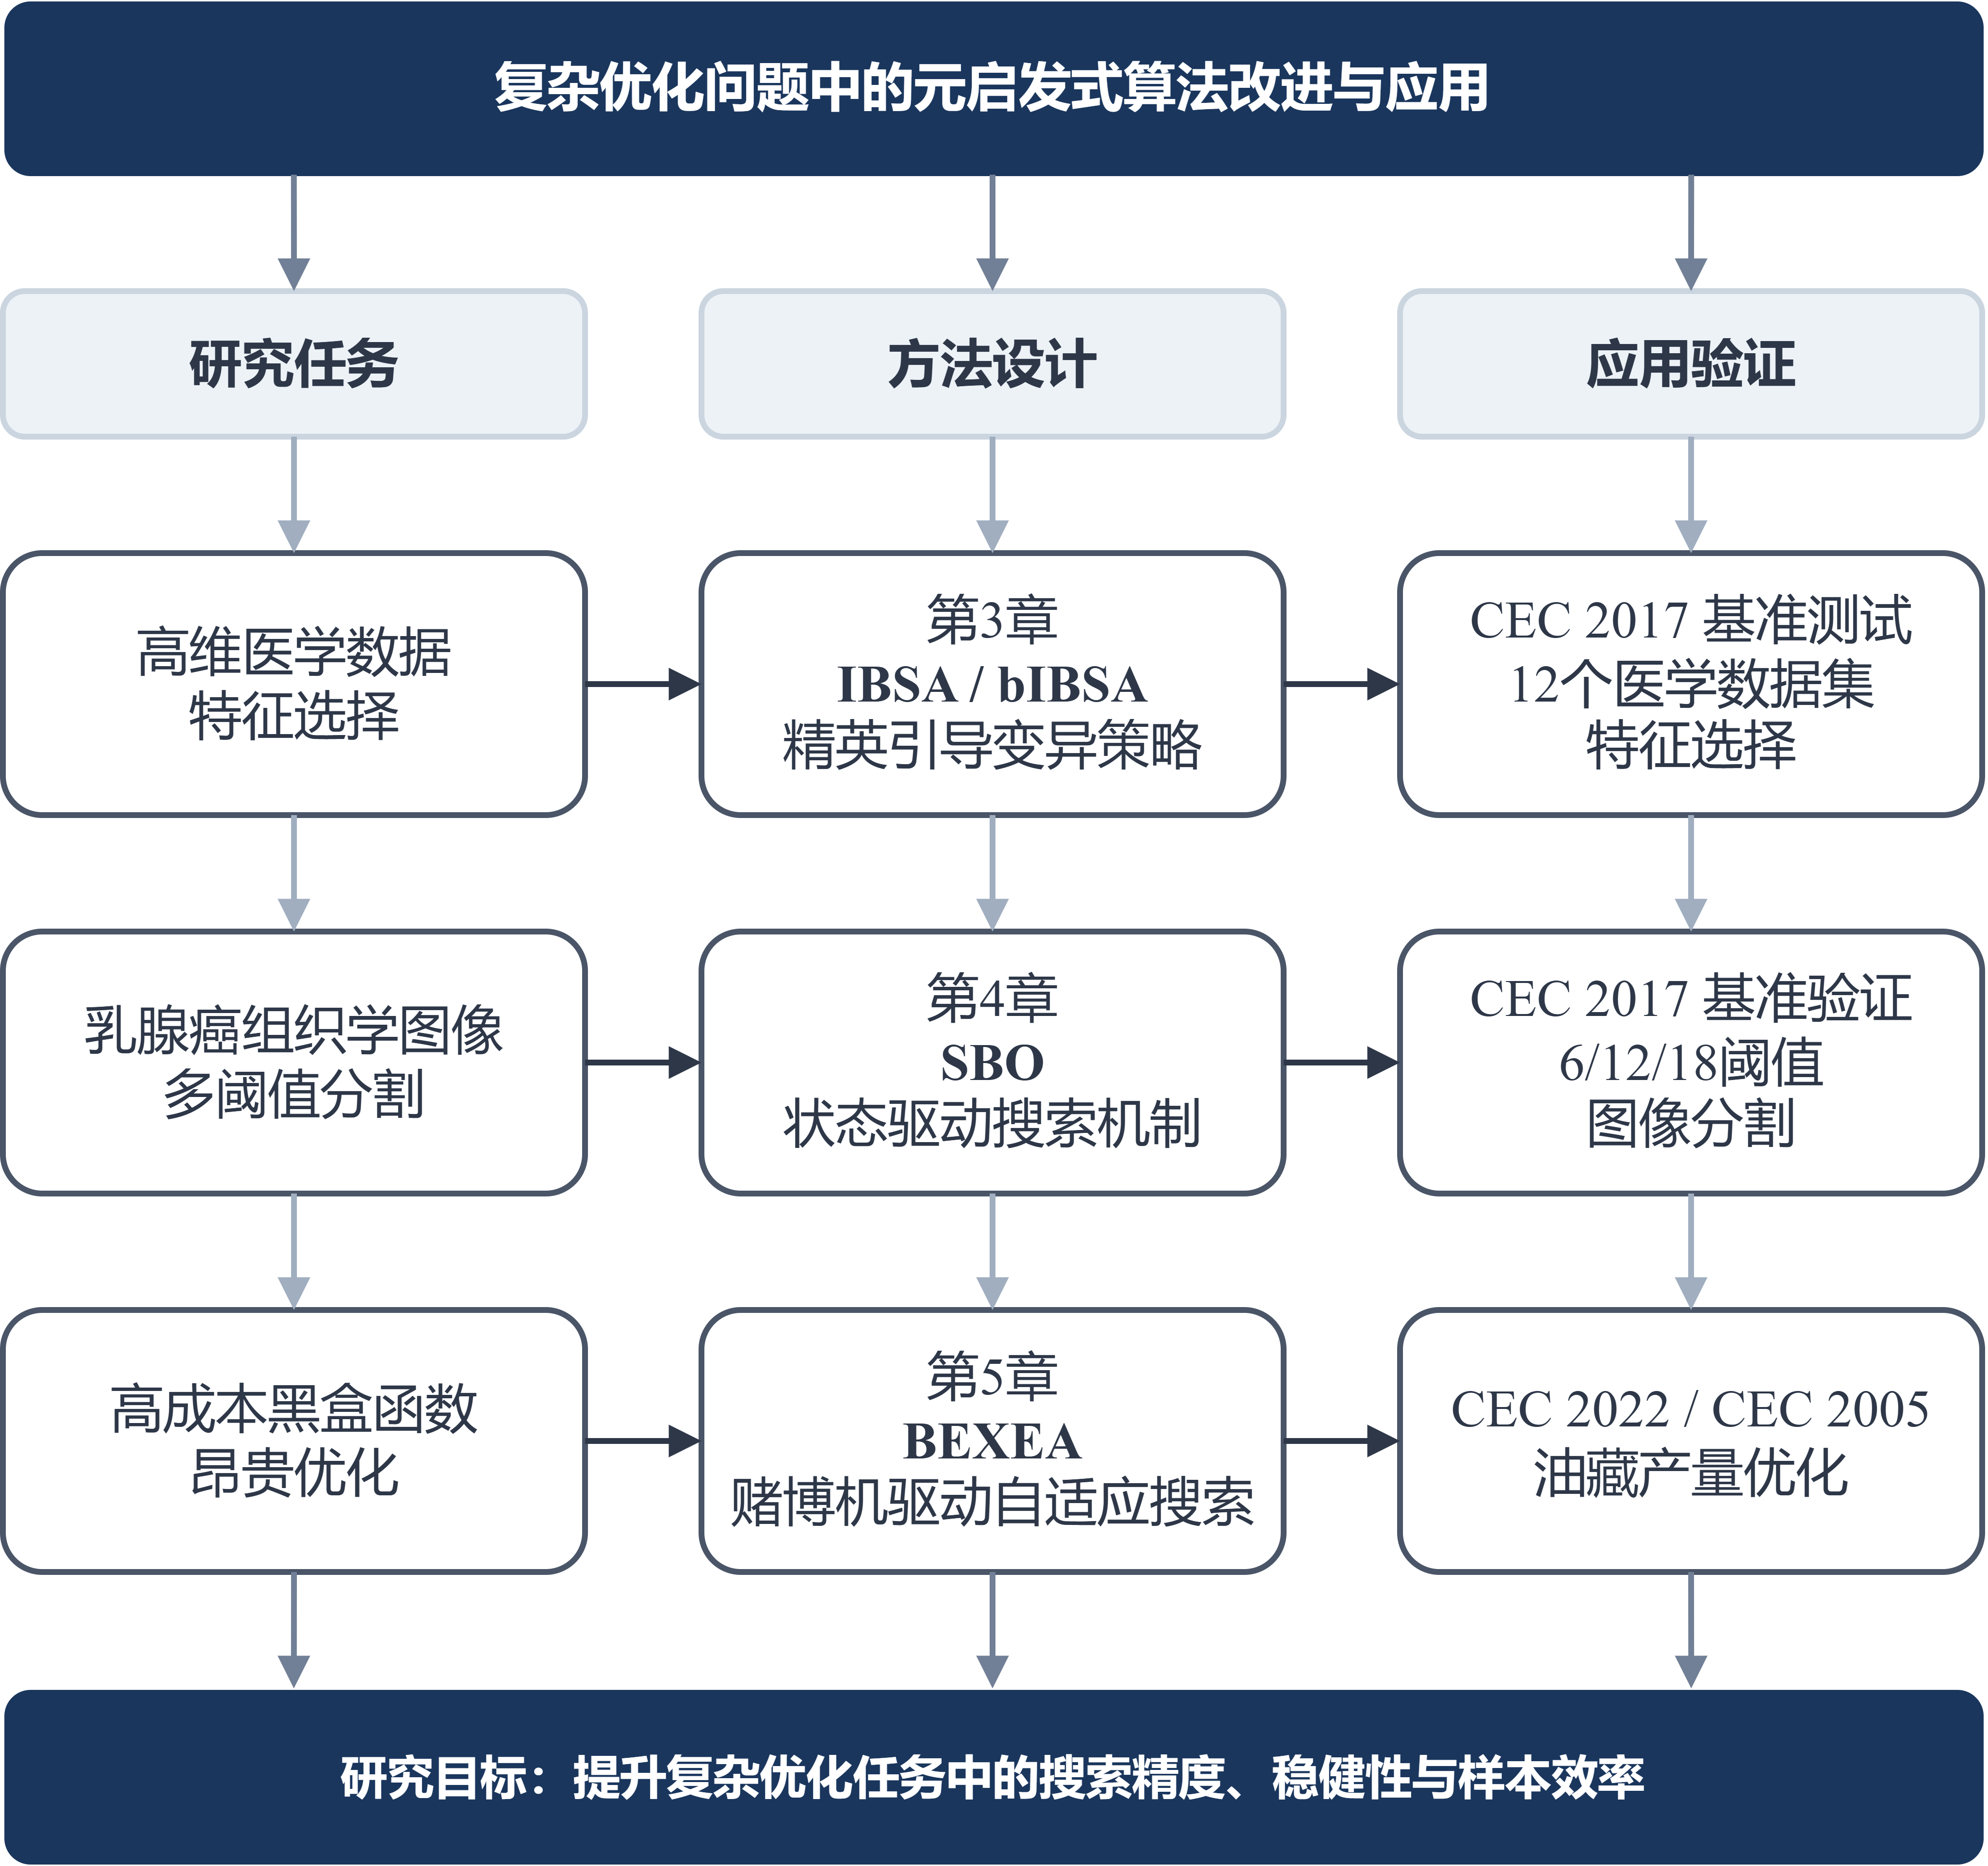
\includegraphics[width=0.96\textwidth]{figures/chapter1/thesis_overview_refined.drawio.png}
  \bicaption{总体技术框架图}{Framework diagram of the overall thesis}
  \label{fig:overall-framework}
\end{figure}

本研究以复杂任务中的共性瓶颈为导向，由三条平行的研究路径支撑：针对特征选择中的平衡性难题，提出IBSA及其离散变体bIBSA；针对图像分割中的策略协调问题，开发状态驱动的SBO算法；针对昂贵优化的效率挑战，构建赌博机驱动的BEXEA架构。各核心章节均遵循“算法建模—基准测评—工程验证”的叙事逻辑，确保论证过程的严密与统一。

从论证脉络看，各章节间并非简单的横向罗列，而是遵循了“既有框架优化、全新机制探索、复杂场景扩展”的演进逻辑。第三章聚焦BSA框架的精英信息挖掘，验证改进策略在多维场景下的适配度；第四章针对复杂连续域的控制难题，由浅入深地推导出全新的SBO算法，以增强状态感知能力；第五章则将视角延展至高成本优化领域，结合前序搜索机制，引入代理模型与赌博机决策，形成应对极低评估预算的BEXEA方案。

\section{本文组织结构安排}

本研究围绕特征选择、图像分割及昂贵优化三类典型任务，重点探讨元启发式算法的优化机理及其在工程中的应用实践。全文在阐明背景现状的基础上，分层次论述了三种改进算法的设计初衷、数学表征及应用效能。具体安排如下：

第一章，绪论：阐述课题背景与意义，评述国内外研究动态，并给出整体研究架构与章节脉络。

第二章，相关理论及技术：梳理后续研究的理论根基，包括元启发式搜索范式、应用场景数学建模、代理辅助技术、赌博机博弈理论及统计测评体系。

第三章，基于精英引导变异策略的改进回溯搜索算法：针对BSA在精英利用上的滞后问题，详细阐述IBSA的设计机理及其变异策略。通过基准函数测评与高维医学数据集筛选任务，验证其在精度与稀疏性上的优势。

第四章，基于状态的优化算法：针对复杂连续域寻优中的协调难题，推出全新的SBO算法，系统论证其状态驱动机制的科学性，并结合乳腺癌组织图像分割任务验证其实用价值。

第五章，基于赌博机驱动的自适应搜索代理辅助进化算法：面向评估预算高度受限的场景，论述BEXEA的自适应搜索策略与不确定性采样准则。通过标准昂贵优化测试集与实际油藏产量优化案例，评估其样本利用效率。

第六章，总结与展望：提炼主要创新点，剖析研究局限，并对智能优化领域的未来走向进行展望。
��
